\subsection{Representations of Variability Models}

\begin{frame}{\insertsubsection} % show list of cfgs, diagrams, text => what are the problems? 
	% this notation is already nice for communication, but semantics matter (for large models, it does not suffice to look sharply)

	% why is this needed? (forward ref?)

	% this section shall teach the relationship between FMs and formulas and FMs and sets (i.e., Damiani 2020, Batory 2005), so: FM semantics

	% also, (valid) total configurations should be explained here (how a computer can check them, this can be checked easily when an FM is encoded eg as runtime variability, but all other SAT-based questions are hard to answer)

	% recount the example model here

	\leftandright{
		\myexample{Natural Language}{
			\tiny ``A \feat{configurable database} has an API that allows for at least one of the request types \feat{Get}, \feat{Put}, or \feat{Delete}.
			Optionally, the database can support \feat{transactions}, provided that the API allows for Put or Delete requests.
			Also, the database targets a supported operating system, which is either \feat{Windows} or \feat{Linux}.''
		}
		\myexample{Configuration Map}{
			\tiny
			\leftandright{
				$\{C,G,W\}$\\
				\hspace{4mm}\vdots\\[1ex]
				$\{C,G,P,D,T,W\}$
			}{
				$\{C,G,L\}$\\
				\hspace{4mm}\vdots\\[1ex]
				$\{C,G,P,D,T,L\}$
			}
		}
		\myexampletight{Feature Model}{
			\centering\tiny
			\featureDiagramConfigurableDatabase
		}
	}{
		\centering
		\usetikzlibrary{positioning}
		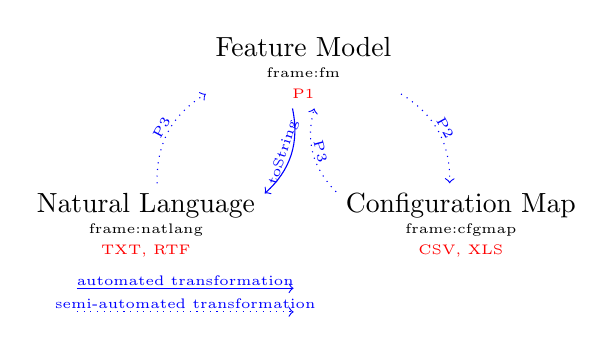
\begin{tikzpicture}
			\tikzstyle{every edge}=[font=\tiny,draw,color=blue]
	
			\node (fd) at (2,0) [align=center] {Feature Model\\[-1ex]\tiny\refslide{frame:fm}\\[-1ex]{\tiny\color{red}P1}};
			\node (nat) at (0,-2) [align=center] {Natural Language\\[-1ex]\tiny\refslide{frame:natlang}\\[-1ex]{\tiny\color{red}TXT, RTF}};
			\node (cfg) at (4,-2) [align=center] {Configuration Map\\[-1ex]\tiny\refslide{frame:cfgmap}\\[-1ex]{\tiny\color{red}CSV, XLS}};
	
			\path [->] (fd) edge[bend left] node[sloped,yshift=1mm] {toString} (nat);
			\path [dotted, ->] (nat) edge[bend left] node[sloped,yshift=1mm] {P3} (fd);
			
			\path [dotted, ->] (fd) edge[bend left] node[sloped,yshift=1mm] {P2} (cfg);
			\path [dotted, ->] (cfg) edge[bend left] node[sloped,yshift=1mm] {P3} (fd);

			\node (trans) at (-1,-2.8) {};
			\node (trans2) at (2,-2.8) {};
			\node (trans3) at (-1,-3.1) {};
			\node (trans4) at (2,-3.1) {};
			\path [->] (trans) edge node[yshift=1mm] {automated transformation} (trans2);
			\path [dotted, ->] (trans3) edge[yshift=5mm] node[yshift=1mm] {semi-automated transformation} (trans4);
		\end{tikzpicture}

		\mynote{Problems}{
			\begin{enumerate}%[label=P\arabic*]
				\item How to express feature models textually?
				\item How to obtain configurations automatically?
    			\item \color{gray}{(How to reverse engineer feature models?)}
			\end{enumerate}
		}
	}
\end{frame}


\subsection{Universal Variability Language}

\begin{frame}{\insertsubsection}
	\leftorright{
		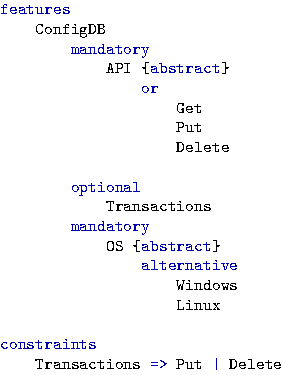
\includegraphics[width=0.7\linewidth]{uvl-model}
	}{
		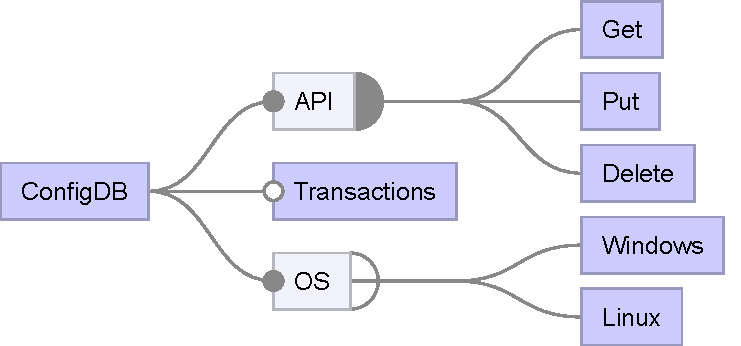
\includegraphics[width=\linewidth]{varied-model}
		\mynote{UVL}{
			\begin{itemize}
				\item textual language for feature modeling
    			\item \todots
			\end{itemize}
		}
	}
\end{frame}

\subsection{Propositional Formulas}

\begin{frame}{\insertsubsection}
	Syntax of formulas

	explain $\pand, \por, \pnot, \pimplies, \pequals$


	here, we do not allow $\forall, \exists$ (extensions exist: QBF (e.g., slicing), FOL (non-Boolean models))
\end{frame}

\begin{frame}{\insertsubsection}
	show running example as a formula
	
	explain intuition behind elements of formula

	motivate very shortly why this might be nice

	there is evidence (Knueppel) that the full expressive power of Boolean formulas is needed for real-world formulas
\end{frame}

\subsection{From Diagram to Formula}

\forestset{
	featureDiagram/.style={
		for tree={
			text depth = 0,
			parent anchor = south,
			child anchor = north,
			draw = drawColor,
			edge = {draw=drawColor},
		}
	}
}

\begin{frame}{-- Algorithm}
	\leftorright{
		$\phi\left(\featureDiagram{Root}\right) = Root$
	
		$\phi\left(\featureDiagram{P[C,optional]}\right) = C \pimplies P$
	
		$\phi\left(\featureDiagram{P[C,mandatory]}\right) = C \pequals P$
	}{
		$\phi\left(\featureDiagram{P[$C_1$,or][\ldots][$C_n$]}\right) = (\bigvee_{1 \leq i \leq n} C_i) \pequals P$
		
		$\phi\left(\featureDiagram{P[$C_1$,or][\ldots][$C_n$]}\right) = (\bigvee_{1 \leq i \leq n} C_i) \pequals P \pand \bigwedge_{1 \leq i < j \leq n} \pnot (C_i \pand C_j)$
	}

\end{frame}

\subsection{Conjunctive Normal Form}

\begin{frame}{-- Conjunctive Normal Form}
	CNF is a universal language for saving Boolean formulas, maybe explain it here?
\end{frame}

\begin{frame}{-- Equivalent Transformation}
	
\end{frame}

\begin{frame}{-- DIMACS File Format}
	
\end{frame}

%(state BDD?)
% probably not - (knowledge compilation: there are many nuances between CNF and BDD, maybe discuss?)

\subsection{Other Representations} %variations? these are not only other representations of the same notation

\begin{frame}{\insertsubsection}
	Extended Feature Models
	
	%at the end (what else is there?): in practice, we also have non-Boolean features/attributes/constraints over attributes (more details on efficiency in third block)

	Cardinalities

	Linux/Kconfig % tri-state features
\end{frame}







% \subsection{Enumerating All Configurations}
% \begin{frame}{\insertsubsection}
% 	\leftandright{
% 		%\myexampletight{}{\centering\includegraphics[width=.75\textwidth]{db-constraint}}
% 		\myexample{26 Valid Configurations}{
% 			\footnotesize
% 			\leftandright{
% 				$\{B,G,W\}$\\
% 				$\{B,P,W\}$\\
% 				$\{B,G,P,W\}$\\
% 				$\{B,D,W\}$\\
% 				$\{B,G,D,W\}$\\
% 				$\{B,P,D,W\}$\\
% 				$\{B,G,P,D,W\}$\\
% 				$\{B,P,T,W\}$\\
% 				$\{B,G,P,T,W\}$\\
% 				$\{B,D,T,W\}$\\
% 				$\{B,G,D,T,W\}$\\
% 				$\{B,P,D,T,W\}$\\
% 				$\{B,G,P,D,T,W\}$
% 			}{
% 				$\{B,G,U\}$\\
% 				$\{B,P,U\}$\\
% 				$\{B,G,P,U\}$\\
% 				$\{B,D,U\}$\\
% 				$\{B,G,D,U\}$\\
% 				$\{B,P,D,U\}$\\
% 				$\{B,G,P,D,U\}$\\
% 				$\{B,P,T,U\}$\\
% 				$\{B,G,P,T,U\}$\\
% 				$\{B,D,T,U\}$\\
% 				$\{B,G,D,T,U\}$\\
% 				$\{B,P,D,T,U\}$\\
% 				$\{B,G,P,D,T,U\}$
% 			}
% 		}
% 	}{}
% \end{frame}

% \subsection{Linux Feature Model}
% \begin{frame}{\insertsubsection}
% 	\vspace{28mm}~\hspace{-15mm}\href{https://dl.acm.org/doi/abs/10.1145/3382025.3414943}{\includegraphics[width=1.2\linewidth,trim=100 510 100 170,clip]{linux-bdd}}
% \end{frame}

% \subsection{Dependencies Modeled in Excel}
% \begin{frame}{\insertsubsection}
% 	\vspace{-7mm}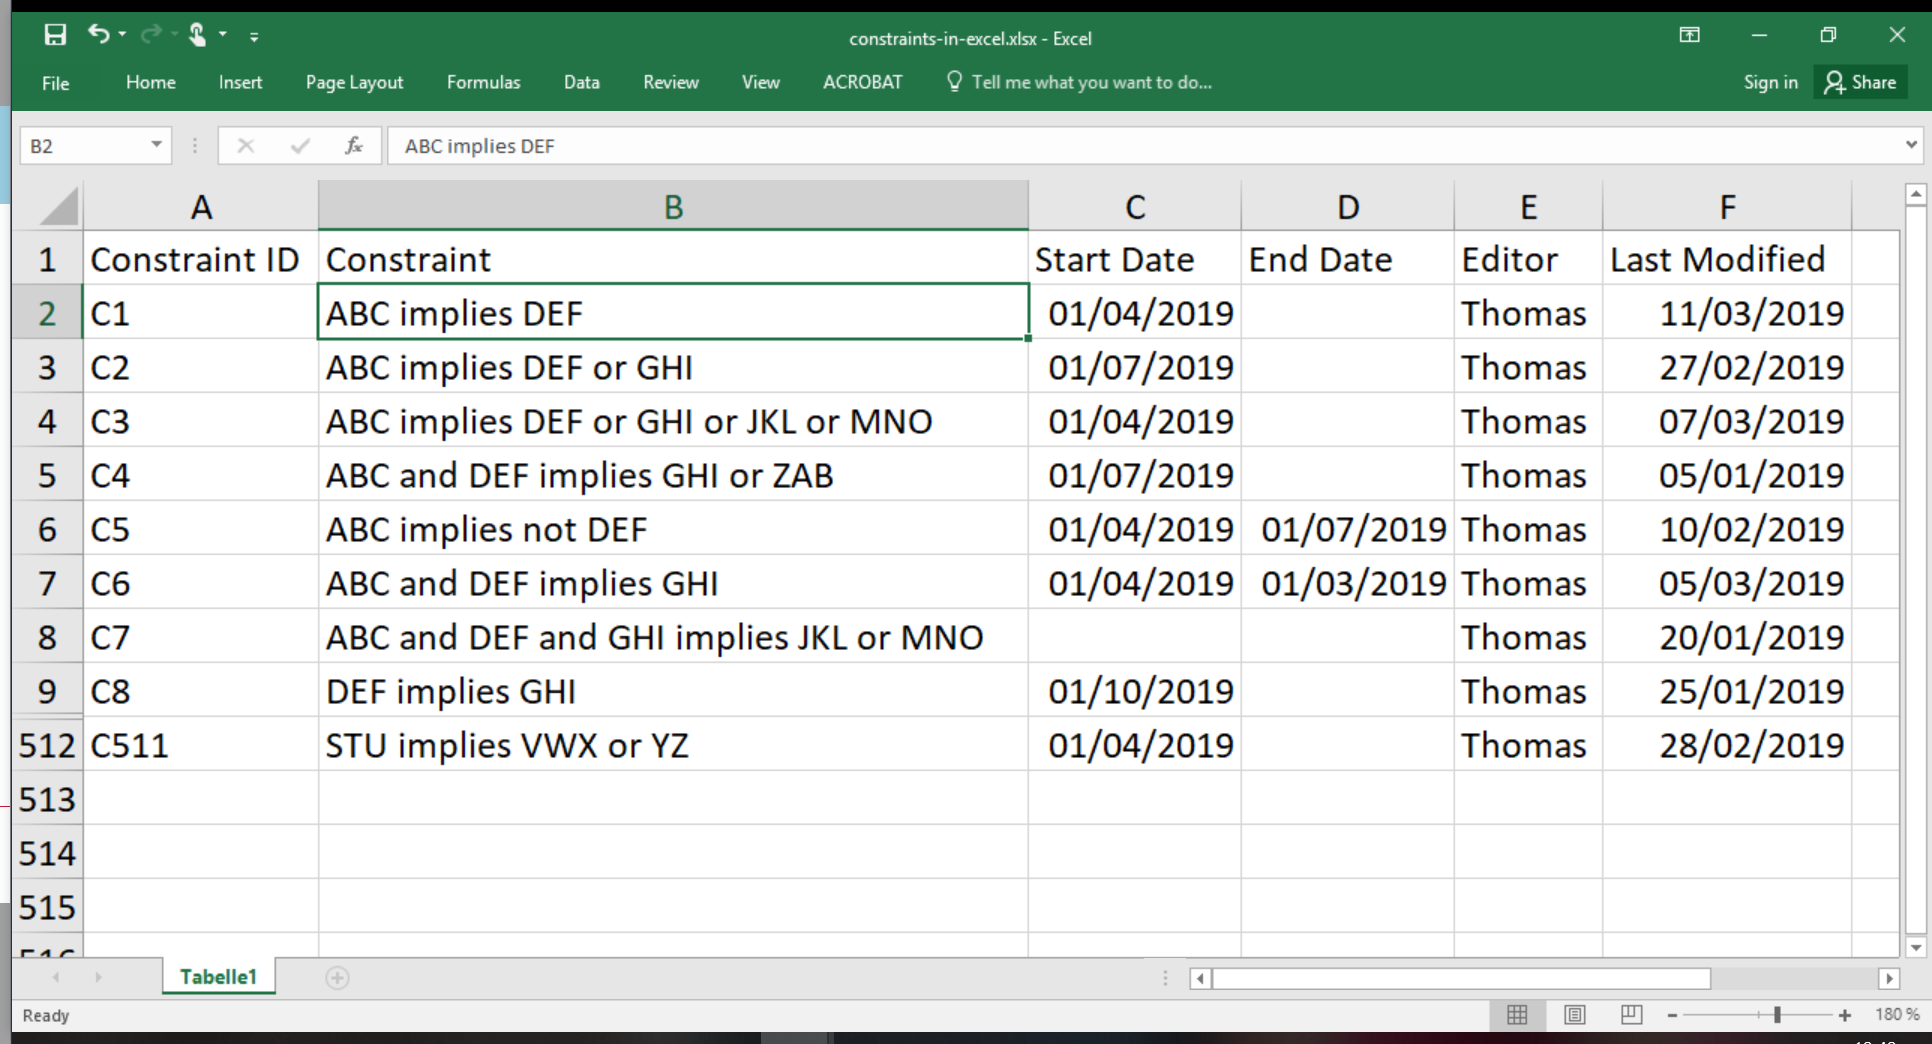
\includegraphics[width=.7\linewidth,trim=10 10 0 10,clip]{constraints-in-excel}
% \end{frame}

\begin{frame}{\insertsubsection}
	\myexampletight{Representations of Variability Models}{
		\usetikzlibrary{positioning}
		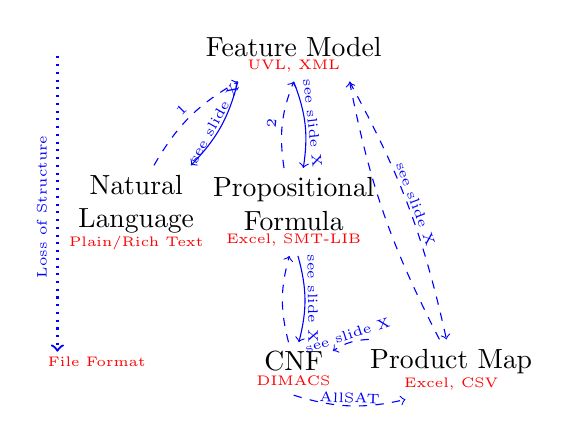
\begin{tikzpicture}
			\tikzstyle{every edge}=[font=\tiny,draw,color=blue]
	
			\node (topleft) at (-1,0) {};
			\node (bottomleft) at (-1,-4) {};
			\node (bottomleft2) at (-0.5,-4) {\tiny\color{red}File Format};
			
			\node (fd) at (2,0) {Feature Model};
			\node (fd2) at (fd.south) {\tiny\color{red}UVL, XML};
			\node (nat) at (0,-2) [align=center] {Natural\\Language};
			\node (nat2) at (nat.south) {\tiny\color{red}Plain/Rich Text};
			\node (phi) at (2,-2) [align=center] {Propositional\\Formula};
			\node (phi2) at (phi.south) {\tiny\color{red}Excel, SMT-LIB};
			\node (cfg) at (4,-4) {Product Map};
			\node (cfg2) at (cfg.south) {\tiny\color{red}Excel, CSV};
			\node (cnf) at (2,-4) {CNF};
			\node (cnf2) at (cnf.south) {\tiny\color{red}DIMACS};
	
			\path [dotted, thick, ->] (topleft) edge node[left, rotate=90, yshift=2mm, xshift=10mm] {Loss of Structure} (bottomleft);
		
			\path [->] (fd2.south west) edge[bend left=15] node[sloped,yshift=1mm] {see slide X} (nat);
			\path [dashed, ->] (nat) edge[bend left=15] node[sloped,yshift=1mm] {\footnote{\bakarnaturallanguage}} (fd2.south west);
			
			\path [->] (fd2.south) edge[bend left=15] node[sloped,yshift=1mm] {see slide X} (phi);
			\path [dashed, ->] (phi) edge[bend left=15] node[sloped,yshift=1mm] {\footnote{\czarneckithereandbackagain, \shereverseengineering}} (fd2.south);

			\path [dashed, ->] (fd2.south east) edge[bend left=8] node[sloped,yshift=1mm] {see slide X} (cfg);
			\path [dashed, ->] (cfg) edge[bend left=8] node[sloped,yshift=1mm] {\todots} (fd2.south east);

			\path [->] (phi2) edge[bend left=15] node[sloped,yshift=1mm] {see slide X} (cnf);
			\path [dashed, ->] (cnf) edge[bend left=15] node[sloped,yshift=1mm] {\todots} (phi2);
		
			\path [dashed, ->] (cfg) edge[bend right=15] node[sloped,yshift=1mm] {see slide X} (cnf);
			\path [dashed, ->] (cnf2.south) edge[bend right=15] node[sloped,yshift=1mm] {AllSAT} (cfg2);
		\end{tikzpicture}

		% describe sat, #sat, allsat
		% describe size of product lines (chico)

		% \myexampletight{Industrial Configuration Spaces \mysource{\evaluatingsharpsatsolvers}}{
		% 	\centering\evaluatingsharpsatsolverslink{\includegraphics[width=\linewidth,page=6,trim=50 210 320 440,clip]{2020/2020-VaMoS-Sundermann}}
		% }

		% feature model of the linux kernel als motivation nutzen, dann recap in testing VL
	}
\end{frame}